\documentclass[aspectratio=43,unicode,10pt]{beamer}
\usetheme{ttipresentation}

\usepackage{luatexja}
\usepackage{graphicx}
\usepackage{calc}
\usepackage[overlay,absolute]{textpos}

\setlength{\TPHorizModule}{\textwidth}
\setlength{\TPVertModule}{\textheight}
\newlength\horizoffset
\setlength{\horizoffset}{1in+\hoffset+\oddsidemargin}
\newlength\vertoffset
\setlength{\vertoffset}{1in+\voffset+\topmargin+\headheight+\headsep}
\textblockorigin{\horizoffset}{\vertoffset}

\beamertemplatenavigationsymbolsempty
\newcommand{\itemtitle}[1]{\textbf{#1}\\}
\newcommand{\fire}[1]{\textcolor{red}{\textbf{#1}}}


\title{文書・文間及びカテゴリ間の関係を\\考慮したレーティング予測}
\institute{知能数理研究室}
\author{12056 外山 洋太}
\date{\today}



\begin{document}

\begin{frame}
\titlepage
\end{frame}

\begin{frame}{研究背景}{}
  \begin{block}{商品レビューによる評判分類}
    \begin{itemize}
      \item 対象問題:複数のカテゴリにおけるレーティング予測
      \item 文字から文書に渡る\fire{様々な言語要素間の関係}、 \\
            及び、\fire{カテゴリ間の関係}が重要
      \item 従来手法はそれらを十分に考慮できていない
    \end{itemize}
  \end{block}
  \begin{figure}
    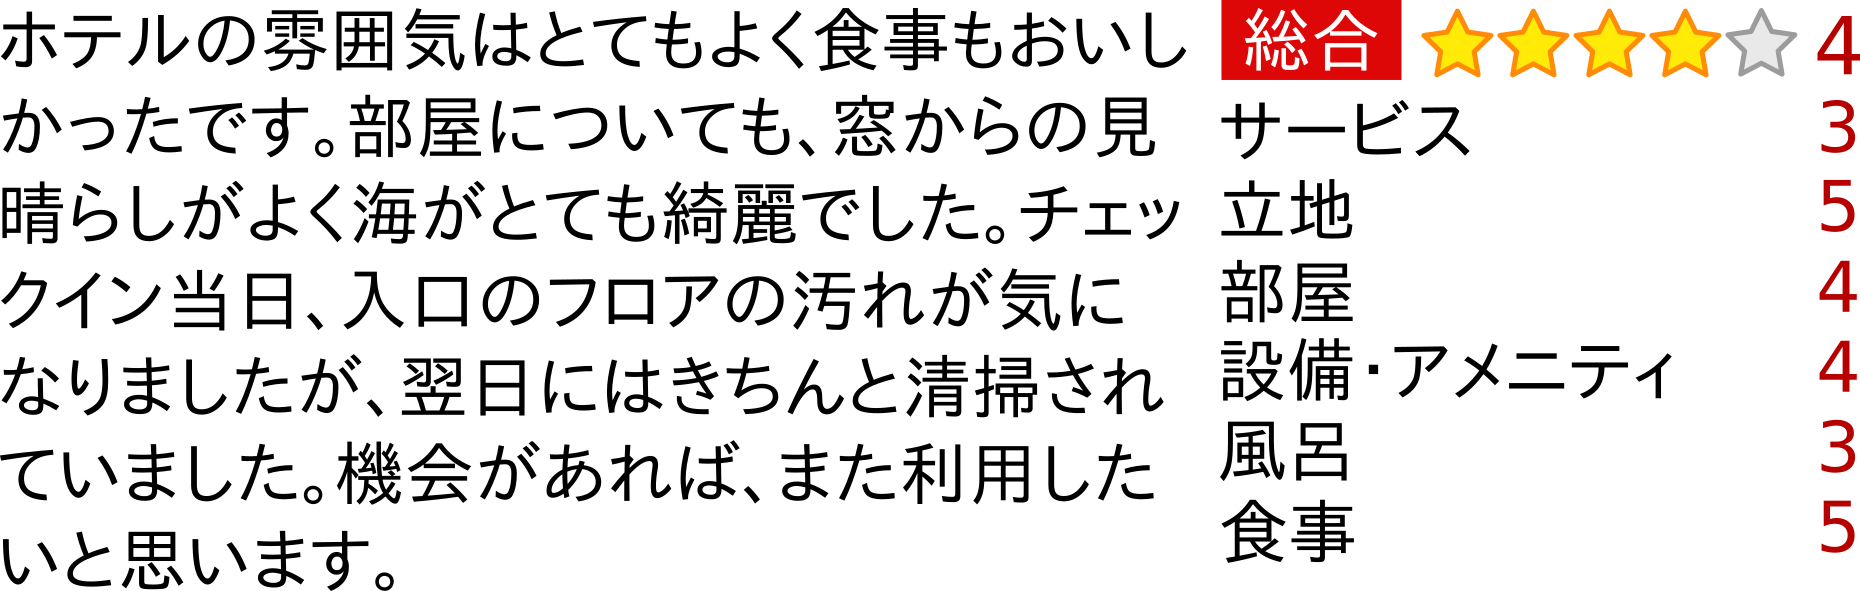
\includegraphics[width=0.7\linewidth]{fig/review.png}
  \end{figure}
\end{frame}

\begin{frame}{提案手法}{}
  \begin{block}{目的}
    以下を考慮した分類の実現
    \begin{itemize}
      \item \fire{文章・文間の関係}
      \item \fire{カテゴリ間の関係}
    \end{itemize}
  \end{block}
  \begin{textblock}{0.6}(0.425,0.15)
    \fboxsep=2mm % HACK
    \fcolorbox{white}{white}{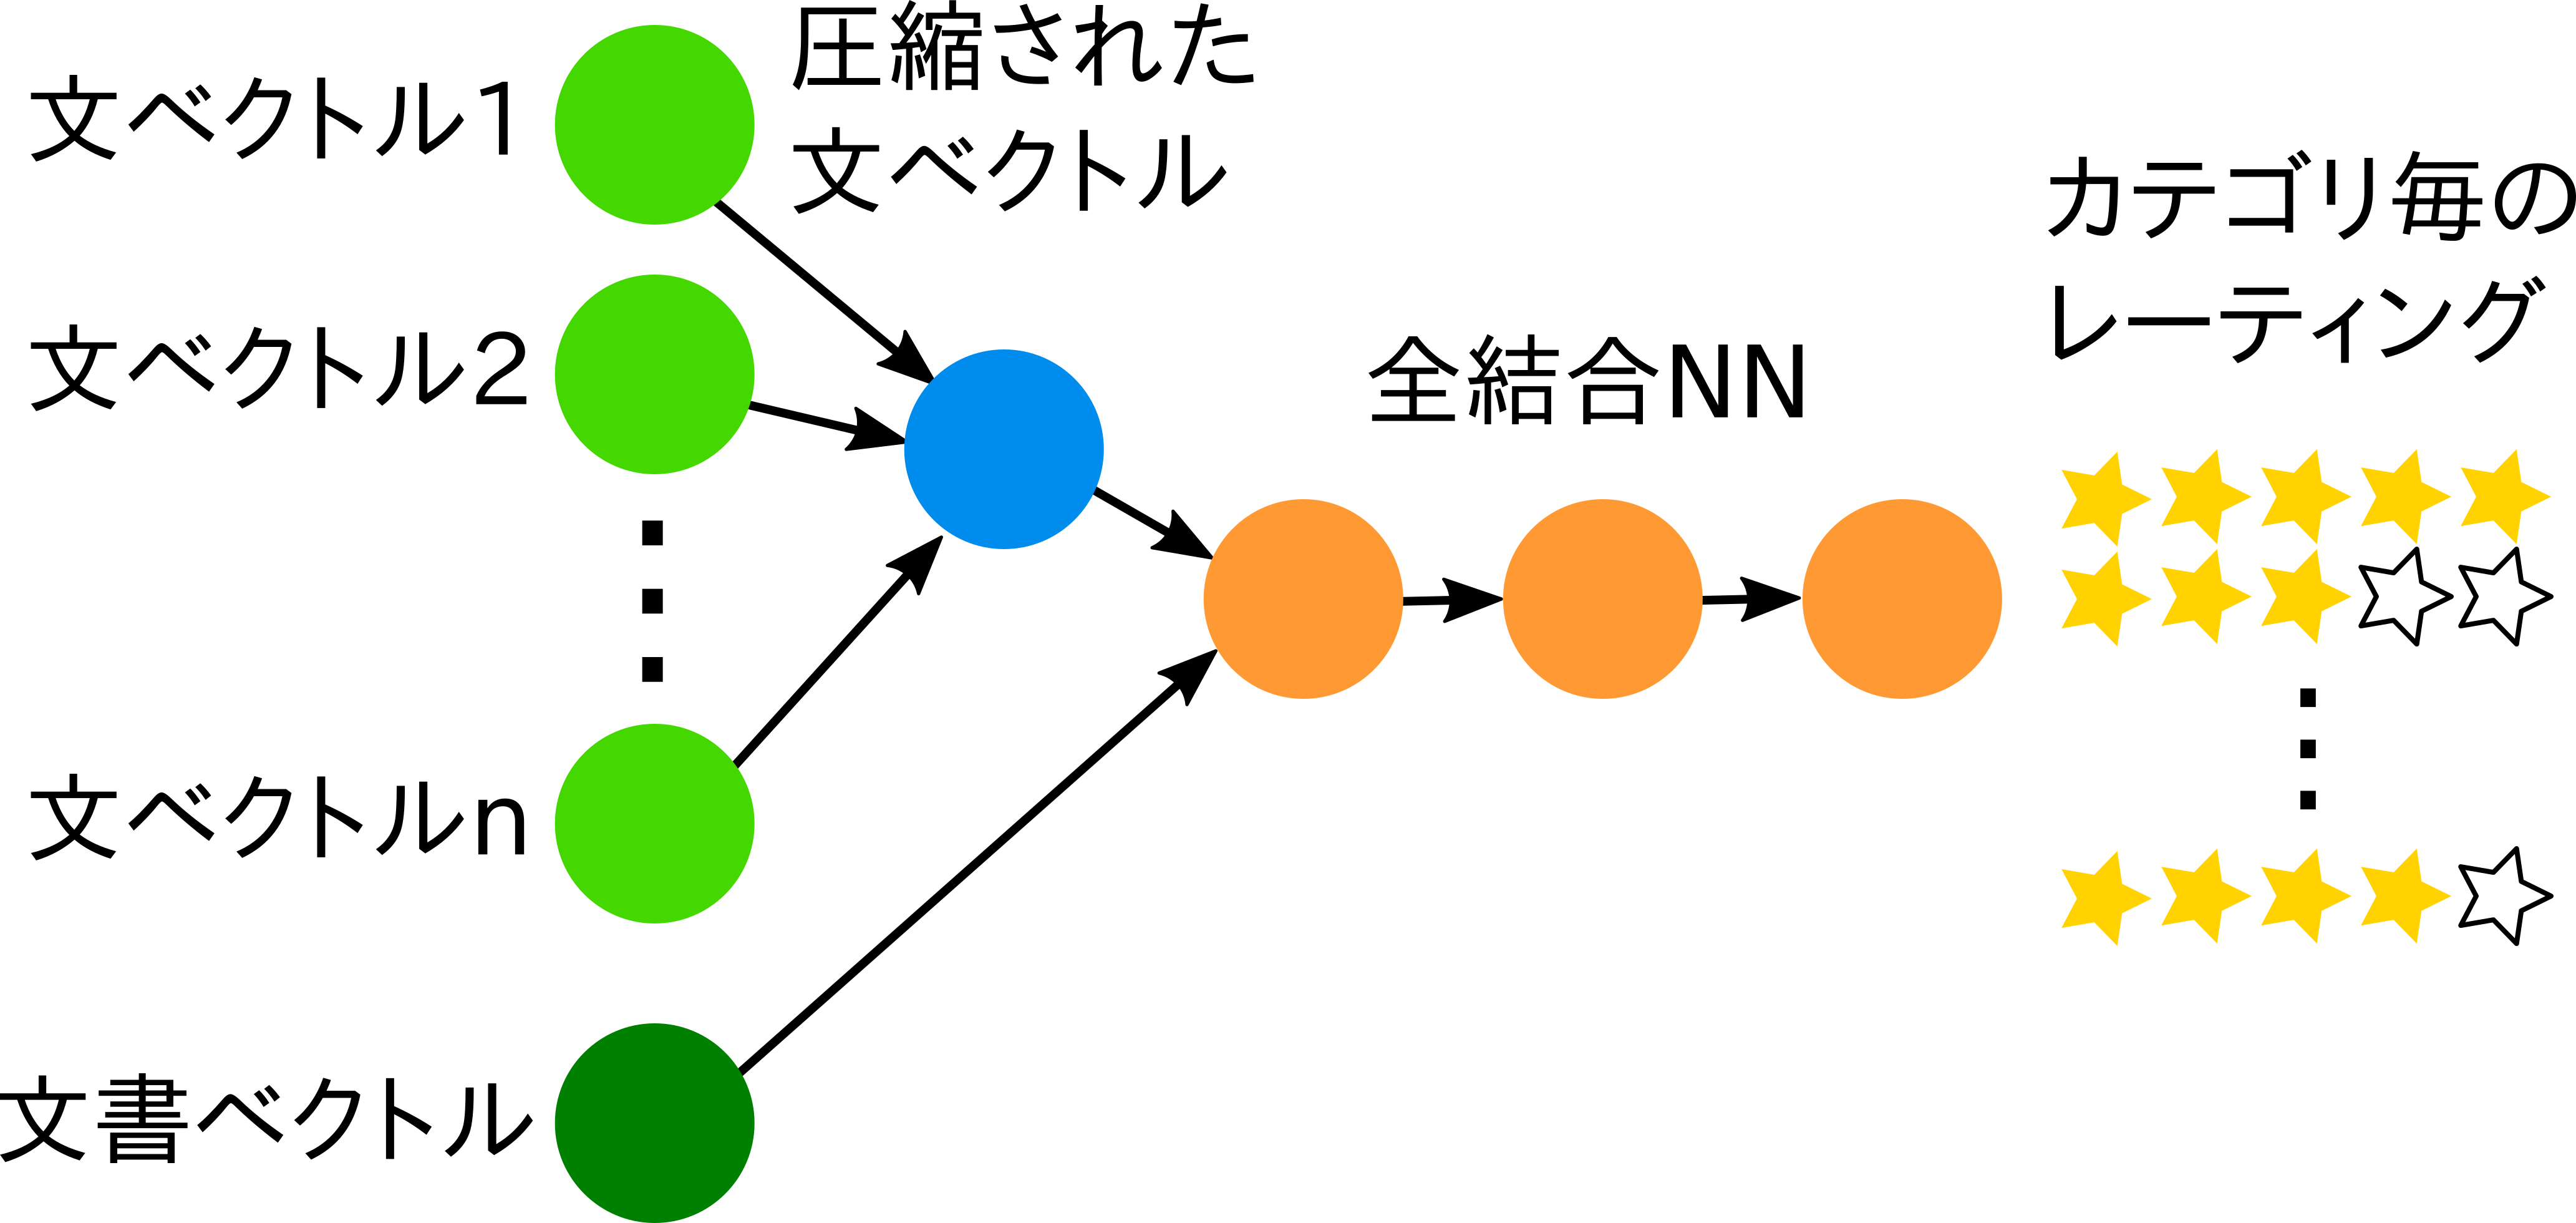
\includegraphics[width=\linewidth]{fig/model.png}}
  \end{textblock}
  \begin{block}{方法}
    \begin{itemize}
      \item \itemtitle{パラグラフベクトル}
        \begin{itemize}
          \item 文や文書を、その意味を表す実数ベクトルに変換する手法
          \item \fire{評判分類において優れる}
        \end{itemize}
      \item \itemtitle{ニューラルネットワーク}
        \begin{itemize}
          \item 神経回路を模した機械学習手法
          \item 分類問題に適用可能
          \item \fire{文書・文間やカテゴリ間の複雑な関係}を考慮
        \end{itemize}
    \end{itemize}
  \end{block}
\end{frame}

\begin{frame}{実験及び結果}{}
  \begin{block}{実験設定}
    \begin{itemize}
      \item 7カテゴリ6クラスのレーティング予測の正答率を測定
      \item データセット:楽天トラベルにおけるレビュー約330,000件
    \end{itemize}
  \end{block}
  \begin{block}{結果}
    %\begin{columns}[onlytextwidth,t]
      %\begin{column}{0.6\linewidth}
        \begin{itemize}
          \item 提案手法が従来手法より\fire{高い正答率}を示す
          \item \fire{文の並び}が予測のために重要
          \item 文書ベクトルと文ベクトルを同時に素性として用いることが有効
        \end{itemize}
      %\end{column}
      %\begin{column}{0.4\linewidth}
        \begin{table}
          \centering
          \begin{tabular}{l | r} \label{tab:Accuracies}
            手法 & 正答率 \\
            \hline
            従来手法 & 0.4832 \\
            提案手法 & \fire{0.5030} \\
          \end{tabular}
        \end{table}
      %\end{column}
    %\end{columns}
  \end{block}
\end{frame}

\end{document}
